\section{族内更新的实施}
\label{sec:igeo-implementation}

把自然梯度用到第~\ref{chap:distribution-approximation}章的逼近目标上，每一步要做四件事：算出目标的梯度，得到Fisher信息或它与向量的乘积，解一个线性方程得到方向，再定步长并保证新参数仍然合法。前两件常常只能近似完成，后两件则决定了算法在有限步时的表现。

\paragraph{主要思想}
由定义~\ref{def:igeo-natural-gradient}，方向$\bm{d}=\bm{G}^{-1}\bm{g}$。实际计算从不形成逆矩阵，而是解线性方程。为了在$\bm{G}$接近奇异时仍能求解，可以加上一个小的非负数$\gamma$，于是第$t$轮的方向与更新为
\begin{equation}
  \bigl(\bm{G}(\bm{\theta}^{(t)})+\gamma\bm{I}\bigr)\bm{d}^{(t)}=\nabla L(\bm{\theta}^{(t)}),\qquad
  \bm{\theta}^{(t+1)}=\bm{\theta}^{(t)}-\alpha_{t}\,\bm{d}^{(t)}.
  \label{eq:igeo-ngd-update}
\end{equation}
$\gamma=0$时这就是自然梯度步。$\gamma>0$时，$-\bm{d}^{(t)}$是二次模型
\[
  \langle\bm{g},\bm{\delta}\rangle+\frac12\bm{\delta}^{\top}(\bm{G}+\gamma\bm{I})\bm{\delta}
\]
的最小点，相当于在Fisher二次型之外再对参数的欧氏长度加一点惩罚；上一节已经说明，它只是数值上的保护，不能代替对退化方向的分析。

梯度从哪里来，取决于目标的形式。以
\[
  L(\bm{\theta})=D_{\mathrm{KL}}(Q_{\bm{\theta}}\Vert\Pi)=\int q_{\bm{\theta}}\ln\frac{q_{\bm{\theta}}}{\pi}\,\mathrm{d}\nu
\]
为例，$q_{\bm{\theta}}$与$\pi$是相对$\nu$的密度。在积分号下求导需要的条件由第~\ref{chap:expectation-gradient-estimation}章讨论；条件满足时，对被积函数$q_{\bm{\theta}}\ln q_{\bm{\theta}}-q_{\bm{\theta}}\ln\pi$求导，再利用“密度的梯度等于密度乘以得分”与式~\eqref{eq:igeo-score-mean}，得到
\[
  \begin{aligned}
    \nabla L(\bm{\theta})&=\int\nabla q_{\bm{\theta}}\ln\frac{q_{\bm{\theta}}}{\pi}\,\mathrm{d}\nu+\int\nabla q_{\bm{\theta}}\,\mathrm{d}\nu\\
    &=\mathbb{E}_{\bm{\theta}}\Bigl[\bm{s}_{\bm{\theta}}(X)\ln\frac{q_{\bm{\theta}}(X)}{\pi(X)}\Bigr].
  \end{aligned}
\]

在指数族中，由式~\eqref{eq:igeo-expfam-score}，这是$\operatorname{Cov}_{\bm{\theta}}(\bm{T},\ln q_{\bm{\theta}}-\ln\pi)$。若$\Pi$也属于这个族，自然参数为$\bm{\theta}_{\Pi}$，则
\[
  \ln q_{\bm{\theta}}-\ln\pi=\langle\bm{\theta}-\bm{\theta}_{\Pi},\bm{T}\rangle+\text{常数},
\]
于是梯度与自然梯度分别是
\[
  \nabla L(\bm{\theta})=\bm{G}(\bm{\theta})(\bm{\theta}-\bm{\theta}_{\Pi}),\qquad\bm{G}(\bm{\theta})^{-1}\nabla L(\bm{\theta})=\bm{\theta}-\bm{\theta}_{\Pi}.
\]

指数族的自然参数中还有一个省去解方程的办法。目标若写成均值参数的函数，由链式法则与$\partial\bm{m}/\partial\bm{\theta}=\bm{G}$，
\[
  \nabla_{\bm{\theta}}L=\bm{G}(\bm{\theta})\,\nabla_{\bm{m}}L,\qquad\text{从而}\qquad\bm{G}(\bm{\theta})^{-1}\nabla_{\bm{\theta}}L=\nabla_{\bm{m}}L .
\]
在自然参数上走自然梯度步，等于用均值坐标中的普通梯度去更新自然参数。均值坐标下的目标容易求导时，这一形式最省事。

步长分两层控制。第一层是局部预算：由定理~\ref{thm:igeo-steepest}，步长$\alpha$对应的局部KL约为$\frac12\alpha^{2}\,\bm{g}^{\top}\bm{d}$，要它不超过$\varepsilon$，取
\[
  \alpha\leq\sqrt{2\varepsilon/(\bm{g}^{\top}\bm{d})} .
\]
第二层是实际检查：新参数必须属于$\Theta$（例如高斯族的自然参数要求$\theta_2<0$），并且目标要有足够的下降，例如Armijo条件
\begin{equation}
  L(\bm{\theta}-\alpha\bm{d})\leq L(\bm{\theta})-c\,\alpha\,\bm{g}^{\top}\bm{d},\qquad0<c<1 ;
  \label{eq:igeo-armijo}
\end{equation}
不满足就把$\alpha$减半重试，这种回溯可参考\BookChapterRef{chap:smooth-optimization}{卷五第5章“光滑优化基础”}。量$\bm{g}^{\top}\bm{d}$等于$\bm{g}^{\top}\bm{G}^{-1}\bm{g}$，它是自然梯度在Fisher度量下长度的平方，由上一节，它与坐标无关，适合作为停止判据。

\paragraph{计算过程}
下面沿用上一节的例子：目标$\Pi=\mathcal{N}(0,1)$，候选为高斯族，目标函数为式~\eqref{eq:igeo-running-objective}，在自然参数中计算，梯度与信息矩阵都用精确公式。取$\gamma=0$，试探步长$\alpha=\frac12$，Armijo常数$c=10^{-4}$，停止阈值$\mathrm{tol}=10^{-3}$。目标的自然参数是$\bm{\theta}_{\Pi}=(0,\,-0.5)$。

\needspace{6\baselineskip}
\paragraph{变量}
\begin{itemize}
  \item $\bm{\theta}\in\mathbb{R}^{k}$：当前参数，例中$k=2$，并随时换算出$(\mu,v)$。
  \item $\bm{g}\in\mathbb{R}^{k}$：当前梯度$\nabla L(\bm{\theta})$。
  \item $\bm{G}\in\mathbb{R}^{k\times k}$：当前Fisher信息，例中由式~\eqref{eq:igeo-gauss-natural-fisher}计算。
  \item $\bm{C}\in\mathbb{R}^{k\times k}$：$\bm{G}+\gamma\bm{I}$的Cholesky因子，下三角，用后即弃。
  \item $\bm{d}\in\mathbb{R}^{k}$：方向，解方程~\eqref{eq:igeo-ngd-update}得到。
  \item $\alpha$：本轮步长；$L$：当前目标值；$t$：轮次。
\end{itemize}

\paragraph{初始化}
取起点$\bm{\theta}^{(0)}$并检查它属于$\Theta$，算出$L(\bm{\theta}^{(0)})$，令$t=0$。例中起点为$\mathcal{N}(1,4)$，
\[
  \bm{\theta}^{(0)}=(0.25,\ -0.125),\qquad L^{(0)}=-\ln2+2\approx1.3069 .
\]

\needspace{6\baselineskip}
\paragraph{每轮更新}
在第$t$轮：
\begin{enumerate}
  \item \textbf{求梯度与信息矩阵。}计算$\bm{g}=\nabla L(\bm{\theta}^{(t)})$与$\bm{G}=\bm{G}(\bm{\theta}^{(t)})$。例中第一轮$(\mu,v)=(1,4)$，由式~\eqref{eq:igeo-gauss-natural-fisher}与$\bm{g}=\bm{G}(\bm{\theta}-\bm{\theta}_{\Pi})$，
  \[
    \bm{G}=\begin{bmatrix}4&8\\8&48\end{bmatrix},\qquad\bm{g}=\begin{bmatrix}4&8\\8&48\end{bmatrix}\begin{bmatrix}0.25\\0.375\end{bmatrix}=\begin{bmatrix}4\\20\end{bmatrix}.
  \]

  \item \textbf{解方向。}对$\bm{G}+\gamma\bm{I}$作Cholesky分解$\bm{C}\bm{C}^{\top}$，先解$\bm{C}\bm{y}=\bm{g}$，再解$\bm{C}^{\top}\bm{d}=\bm{y}$；分解失败说明矩阵不是正定的，应回到退化分析，而不是继续。例中第一轮
  \[
    \bm{C}=\begin{bmatrix}2&0\\4&4\sqrt2\end{bmatrix}.
  \]
  前代给出
  \[
    y_1=\frac42=2,\qquad y_2=\frac{20-4\cdot2}{4\sqrt2}=\frac{3}{\sqrt2},
  \]
  回代给出
  \[
    d_2=\frac{y_2}{4\sqrt2}=\frac38,\qquad d_1=\frac{2-4\cdot\frac38}{2}=\frac14,
  \]
  即$\bm{d}=(0.25,\,0.375)$。于是$\bm{g}^{\top}\bm{d}=1+7.5=8.5$。

  \item \textbf{检查停止。}若$\bm{g}^{\top}\bm{d}\leq\mathrm{tol}$，输出$\bm{\theta}^{(t)}$并结束。例中第一轮$8.5>10^{-3}$，继续。

  \item \textbf{试探步长。}令$\bm{\theta}'=\bm{\theta}^{(t)}-\alpha\bm{d}$。若$\bm{\theta}'\notin\Theta$，或式~\eqref{eq:igeo-armijo}不成立，把$\alpha$减半重试；成立则接受$\bm{\theta}^{(t+1)}=\bm{\theta}'$，令$t\leftarrow t+1$。例中第一轮
  \[
    \bm{\theta}'=(0.25,\,-0.125)-\tfrac12(0.25,\,0.375)=(0.125,\ -0.3125),
  \]
  $\theta'_2<0$，可行；换算得$v=1/(2\cdot0.3125)=1.6$，$\mu=0.125\cdot1.6=0.2$，由式~\eqref{eq:igeo-running-objective}，
  \[
    L(\bm{\theta}')=-\tfrac12\ln1.6+\tfrac{1.6+0.04}{2}-\tfrac12\approx0.0850 ,
  \]
  远小于Armijo的界$1.3069-10^{-4}\cdot\frac12\cdot8.5$，接受。
\end{enumerate}

例中第二轮从$\mathcal{N}(0.2,\,1.6)$出发。由式~\eqref{eq:igeo-gauss-natural-fisher}，
\[
  \bm{G}=\begin{bmatrix}1.6&0.64\\0.64&5.376\end{bmatrix},\qquad\bm{\theta}-\bm{\theta}_{\Pi}=\begin{bmatrix}0.125\\0.1875\end{bmatrix},\qquad\bm{g}=\begin{bmatrix}0.32\\1.088\end{bmatrix}.
\]
Cholesky因子与解出的方向是
\[
  \bm{C}\approx\begin{bmatrix}1.265&0\\0.506&2.263\end{bmatrix},\qquad\bm{d}=\begin{bmatrix}0.125\\0.1875\end{bmatrix},
\]
其中$C_{2,2}=\sqrt{5.376-0.506^{2}}\approx2.263$。于是
\[
  \bm{g}^{\top}\bm{d}=0.04+0.204=0.244 .
\]
它仍大于阈值。试探步为
\[
  \bm{\theta}'=(0.125,\,-0.3125)-\tfrac12(0.125,\,0.1875)=(0.0625,\ -0.40625),
\]
可行，对应$\mathcal{N}(\frac1{13},\frac{16}{13})$，目标值约$0.0145$，满足式~\eqref{eq:igeo-armijo}，接受。

此后每一轮都重复同样的计算。表~\ref{tab:igeo-ngd-rounds}列出各轮的结果。每轮的$\bm{d}$都等于$\bm{\theta}-\bm{\theta}_{\Pi}$，于是
\[
  \bm{\theta}^{(t)}-\bm{\theta}_{\Pi}=2^{-t}\bigl(\bm{\theta}^{(0)}-\bm{\theta}_{\Pi}\bigr).
\]
第$5$轮开始时$\bm{g}^{\top}\bm{d}\approx3.5\times10^{-4}$，已低于阈值$10^{-3}$，算法停止。最终得到
\[
  \bm{\theta}^{(5)}=\Bigl(\frac1{128},\,-\frac{125}{256}\Bigr),
\]
即$\mathcal{N}(0.008,\,1.024)$，目标值约$1.7\times10^{-4}$。

\begin{BookInlineTable}
  \centering
  \caption{自然梯度迭代的各轮结果，$\alpha=\frac12$，起点$\mathcal{N}(1,4)$，目标$\mathcal{N}(0,1)$。$\bm{g}^{\top}\bm{d}$是本轮开始时自然梯度长度的平方，用于停止判据。}
  \label{tab:igeo-ngd-rounds}
  \begin{tabular}{rrrrr}
    \toprule
    $t$ & $\mu$ & $v$ & $L$ & $\bm{g}^{\top}\bm{d}$ \\
    \midrule
    0 & 1 & 4 & 1.3069 & 8.5 \\
    1 & 0.2 & 1.6 & 0.0850 & 0.244 \\
    2 & 0.0769 & 1.2308 & 0.0145 & 0.0339 \\
    3 & 0.0345 & 1.1034 & 0.00310 & 0.00666 \\
    4 & 0.0164 & 1.0492 & 0.00072 & 0.00149 \\
    5 & 0.0080 & 1.0240 & 0.00017 & 0.00035 \\
    \bottomrule
  \end{tabular}
\end{BookInlineTable}

在这个例子里，若取$\alpha=1$，第一步就直接到达$\bm{\theta}_{\Pi}$。这是因为目标在族内、族是指数族、又在自然参数中计算，三者同时成立时自然梯度恰为$\bm{\theta}-\bm{\theta}_{\Pi}$；一般的逼近问题没有这样的巧合。

\paragraph{算法分析}
先与普通梯度比较。同一个问题在自然参数中用普通梯度，起点处$\bm{g}=(4,20)$，若也取$\alpha=\frac12$，第一步落到$\bm{\theta}=(-1.75,\,-10.125)$，方差约$0.049$，远远越过目标。要避免这种越过，步长要小到约$0.02$；此后在最优点附近，目标的Hessian等于那里的信息矩阵$\operatorname{diag}(1,2)$，每步只把误差缩小约$2\%$。在$(\mu,v)$坐标中用普通梯度、$\alpha=\frac12$，则可以稳定收敛，只是前期较慢。图~\ref{fig:igeo-ngd-runs}对照了三者：普通梯度的表现取决于选哪套坐标，自然梯度的方向则不依赖于这一选择。

\begin{BookInlineFigure}
  \centering
  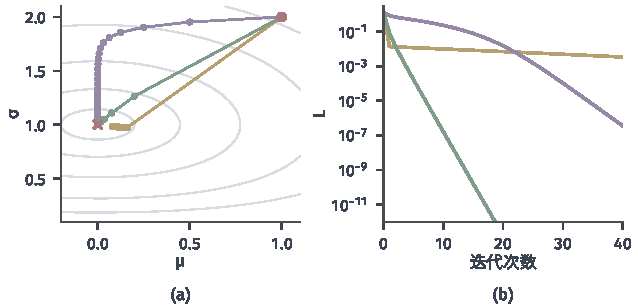
\includegraphics[width=108mm]{figures/07-probability/07-distribution-optimization/matplotlib/igeo-ngd-runs/figure.pdf}
  \caption{从$\mathcal{N}(1,4)$（红点）逼近$\mathcal{N}(0,1)$（红叉），目标$D_{\mathrm{KL}}(Q\Vert\Pi)$，各迭代$40$轮。绿：自然梯度，$\alpha=\frac12$；黄：自然参数中的普通梯度，$\alpha=0.02$；紫：$(\mu,v)$坐标中的普通梯度，$\alpha=\frac12$。(a)迭代点画在$(\mu,\sigma)$平面上，浅灰线为目标的等值线；(b)目标值随迭代次数的变化，纵轴为对数刻度。}
  \label{fig:igeo-ngd-runs}
\end{BookInlineFigure}

收敛方面，表~\ref{tab:igeo-ngd-rounds}的线性收敛是例子的特殊结构给出的。一般情形下，若$L$在非退化的最小点$\bm{\theta}^{*}$附近二阶光滑、$\bm{G}$正定且连续，步长适当时迭代在$\bm{\theta}^{*}$附近线性收敛，速率由$\bm{G}(\bm{\theta}^{*})^{-1}\nabla^{2}L(\bm{\theta}^{*})$的特征值决定；当这个矩阵接近单位阵时，例如目标在族内且用$D_{\mathrm{KL}}(Q\Vert\Pi)$，取$\alpha$接近$1$可以接近Newton法的速度。这只是局部的结论：离最优点很远时，Fisher度量对$L$的曲率没有任何保证，仍要靠回溯和可行性检查。

信息矩阵常常只能估计。由式~\eqref{eq:igeo-fisher}，可以从当前候选分布$Q_{\bm{\theta}}$抽取$n$个独立样本$X_1,\dots,X_n$，用
\begin{equation}
  \widehat{\bm{G}}=\frac1n\sum_{i=1}^{n}\bm{s}_{\bm{\theta}}(X_i)\bm{s}_{\bm{\theta}}(X_i)^{\top}
  \label{eq:igeo-fisher-estimate}
\end{equation}
代替。样本必须来自$Q_{\bm{\theta}}$本身：若改用目标分布的样本计算$\bm{s}_{\bm{\theta}}\bm{s}_{\bm{\theta}}^{\top}$的平均，得到的是得分外积在$\Pi$下的期望，常称为\term{经验Fisher矩阵}（empirical Fisher matrix），除非$Q_{\bm{\theta}}=\Pi$，它不等于$\bm{G}(\bm{\theta})$，所得方向也不再是自然梯度。估计误差按Monte Carlo的速率$n^{-1/2}$缩小，误差分析与方差控制分别见第~\ref{chap:monte-carlo-integration-error}章和第~\ref{chap:variance-reduction}章，梯度本身的随机估计见第~\ref{chap:expectation-gradient-estimation}章。

图~\ref{fig:igeo-fisher-estimate}在例子的起点$\mathcal{N}(1,4)$处做了这一估计。梯度取精确值，$\widehat{\bm{G}}$由$n$个样本得到，方向误差以Fisher范数相对计量。$n=20$时相对误差超过$1$，方向几乎不可信；$n=2000$时约为$8\%$。样本少时，$\widehat{\bm{G}}$的小特征值估计不稳，加上$\gamma$可以避免方向被放大到不合理的长度。

\begin{BookInlineFigure}
  \centering
  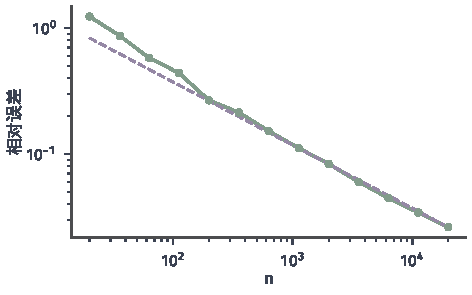
\includegraphics[width=80mm]{figures/07-probability/07-distribution-optimization/matplotlib/igeo-fisher-estimate/figure.pdf}
  \caption{在$\mathcal{N}(1,4)$处用$n$个样本估计自然参数坐标下的Fisher信息，所得方向$\widehat{\bm{d}}=\widehat{\bm{G}}^{-1}\bm{g}$的相对误差$\lVert\widehat{\bm{d}}-\bm{d}\rVert_{\bm{G}}/\lVert\bm{d}\rVert_{\bm{G}}$。绿：$500$次重复的均方根，随机种子$728$；紫色虚线：参考斜率$n^{-1/2}$，在$n=20000$处与绿线对齐。}
  \label{fig:igeo-fisher-estimate}
\end{BookInlineFigure}

计算量方面，用$n$个样本形成$\widehat{\bm{G}}$需要$O(nk^{2})$次运算，Cholesky分解需要$O(k^{3})$，可参考\BookChapterRef{chap:direct-linear-solvers}{卷二第12章“线性方程的直接求解”}。参数维数$k$很大时，两者都负担不起。注意到方程只需要矩阵与向量的乘积，而
\[
  \bm{G}\bm{u}=\mathbb{E}_{\bm{\theta}}\bigl[\bm{s}_{\bm{\theta}}(X)\,\langle\bm{s}_{\bm{\theta}}(X),\bm{u}\rangle\bigr]
\]
可以用同一批样本以$O(nk)$的代价得到，于是可以用共轭梯度法只通过这种\term{Fisher向量积}（Fisher-vector product）近似求解，不必形成$\bm{G}$，可参考\BookChapterRef{chap:krylov-methods}{卷二第15章“Krylov子空间法”}。共轭梯度迭代几步就停止，得到的是近似方向；也可以把$\bm{G}$近似为对角或分块对角矩阵。这些近似都改变了方向，需要用目标值的实际下降来检验。

最后，式~\eqref{eq:igeo-ngd-update}的“在坐标中相加”只是从切向量回到参数空间的一种规则。上一节已经看到，换一套坐标，有限步会到达不同的分布；而参数域的边界，例如方差必须为正，也要单独处理。改用无约束的坐标（如$\tau=\ln v$）、沿测地线移动、或采用满足一阶条件的回缩，都是可选的办法。Fisher度量下的Riemann梯度正是自然梯度，流形上的回缩、向量传输与收敛分析可参考\BookChapterRef{chap:manifold-optimization}{卷五第25章“流形优化”}。

局部几何给出的是方向与尺度，它不代替其他三项检验：迭代是否在全局上收敛，要看目标本身的性质；信息矩阵估计得是否足够准确，要看样本数与方差；族内最优的分布离目标还有多远，是第~\ref{chap:distribution-approximation}章逼近误差的问题，选择更好的更新方向并不能缩小这一差距。
